\documentclass{article}
\usepackage[utf8]{inputenc}
\usepackage{listings}
\usepackage{graphicx}
\usepackage{float}
\usepackage{hyperref}
\usepackage{color}
\usepackage{geometry}



\lstset{
    language=python,
    basicstyle=\footnotesize,
    frame=single,
    keywordstyle=\color{blue}
    }

\title{Rapport Réseau \\
    \large Morpion à l'aveugle
}
\author{Noël Combarieu}
\date{Dimanche 11 novembre 2022}
\geometry{
    top = 20mm,
}
\begin{document}

\maketitle
\newpage
\section{Présentation du projet}
\subsection{Fonctionnement du morpion à l'aveugle}
Le morpion aveugle est une variante de ce jeu dans laquelle les joueurs ne voient pas les coups joués
par l’adversaire. Si un joueur essaie de marquer une case déjà marquée par l’adversaire, le joueur est
informé que cette case est prise et il doit marquer une autre case. \\

\begin{center}
    \begin{figure}[H]
        \begin{center}
            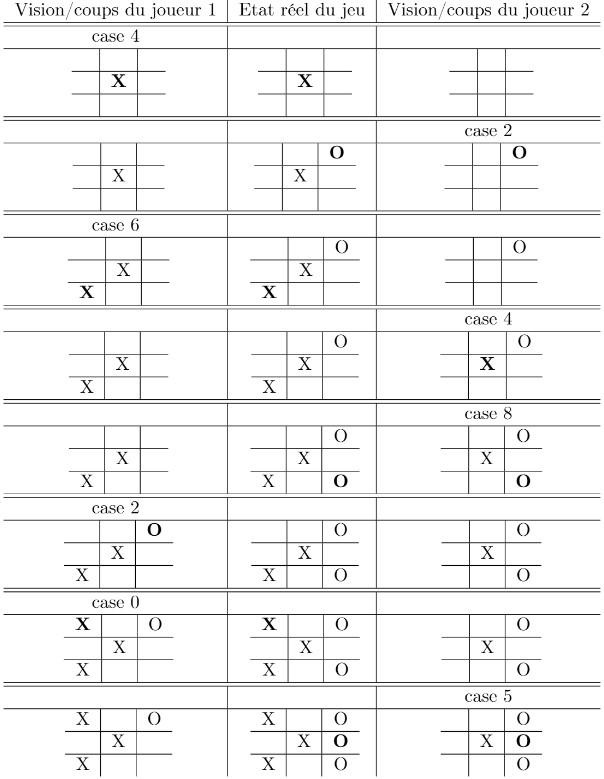
\includegraphics[scale=0.8]{Morpion_aveugle.jpg}
            \caption{Fonctionnement d'un morpion à l'aveugle}
            \label{Pres}
        \end{center}
    \end{figure}
\end{center}

\subsection{Informations relatives au projet}
Le projet est diponible sur mon GitHub :
\url{https://github.com/NCombarieu/Morpion} \\
Le projet a été réalisé en Python 3.9.1 \\

\section{Fonctionnalités du morpion à l'aveugle}
Dans ce morpion à l'aveugle, il y a plusieurs fonctionnalités que j'ai implémenté.

\subsection{Jouer en réseau}
Le joueur peut jouer en réseau avec un autre joueur. Il suffit de démarrer le serveur et de lancer le client en renseignant l'IP et le port à utiliser. \\
Dans notre cas IP = localhost et PORT = 50000 \\\\
Le serveur et le client communiquent via des sockets en TCP. \\\\
Les données du serveur vers le client sont transmises via un protocole que j'ai mis en place . \\\\
Le serveur envoie des variable mot clef au client pour lui indiquer ce qu'il
doit executer.\\
J'ai ainsi le fichier constants.py qui contient les variables mot clef.\\
Exemple : le serveur attend le tire du joueur actuel, le serveur envoie au client le mot clef "GET\textunderscore CLIENT\textunderscore SHOT" :\\
\begin{lstlisting}
    #!/usr/bin/python3
    # PATH: server.py
    from constants import *

    def player_shot(current_player):
    """ Ask the player to play and return the case number """
    sc = clients[current_player-1]
    shot = -1
    while shot <0 or shot >=NB_CELLS:
        sc.send(str(GET_CLIENT_SHOT).encode())
        shot = int(sc.recv(1024).decode())
    return shot
\end{lstlisting}
Le client reste à l'ecoute de ce que le serveur lui envoie avec une boucle infinie.\\
Si il reçoit le mot clef "GET\textunderscore CLIENT\textunderscore SHOT", il rentre dans la condition correspondant.\\
\begin{lstlisting}
    #!/usr/bin/python3
    # PATH: client.py
    from constants import *

    while True:
    """ Receive the message from the server """
    # receive action from server
    action = sc.recv(1)

    if action == GET_CLIENT_SHOT:
        sc.send(input("Quelle case voulez-vous jouer ?").encode("utf-8"))
\end{lstlisting}
\newpage
\subsection{Possibilité de rejouer et de quitter}
Une fois la partie terminée, les joueurs peuvent rejouer sans avoir à relancer le programme.\\
Il suffit de repondre par "Y" lorsque le programme demande si on veut rejouer en fin de partie.\\
Si on répond par "N", le programme se ferme.\\

\subsection{Comptage du score}
Le score est affiché en début de partie.\\
Il est incrémenté à chaque fois qu'un joueur gagne une partie.\\
Il faut que les joueurs décident de rejouer pour que le score soit mis a jour.\\

\subsection{Choix du mode de jeu}
/!\textbackslash Le choix du mode de jeu n'est pas encore implémenté /!\textbackslash \\
Le joueur peut choisir entre jouer contre un autre joueur ou contre l'ordinateur. 
\newpage
\section{Présentation du code}
\subsection{Fonctionnement du code}
Le code est divisé en plusieurs fichiers.\\
Le fichier \textbf{server.py} contient le code du serveur.\\
J'ai tout d'abord mis en place la création d'une socket d'écoute pour le serveur avec de la gestion d'erreur.\\
J'ai ensuite initialisé une liste vide qui contiendra les sockets des clients.\\
J'ai ensuite mis en place une boucle infinie qui va permettre d'accepter la connexion de deux clients afin de pouvoir lancer la partie.\\
\begin{lstlisting}
    # Create a TCP/IP socket
    try:
        ss = socket.socket(socket.AF_INET, socket.SOCK_STREAM)
        ss.setsockopt(socket.SOL_SOCKET , socket.SO_REUSEADDR , 1)
    except socket.error as msg:
        print("Erreur de création de la socket : " + str(msg))
        exit()
    
    HOST = 'localhost'
    PORT = 50000
    
    # Bind the socket to the port
    try:
        ss.bind((HOST, PORT))
        ss.listen(2)
    except socket.error as msg:
        print("Erreur de bind ou de listen : " + str(msg))
        exit()
    
    # Define a list to store the clients sockets
    clients = []
    
    print("Serveur en attente de connexion ...")
    while len(clients) < 2:
        """ Wait for 2 clients """
        readl, _, _ = select.select(clients+[ss], [], [])
        for s in readl:
            if s is ss:
                client, addr = s.accept()
                clients.append(client)
                print("Client connecté : " + str(addr))
                s.send(str(NEW_PLAYER).encode())
\end{lstlisting}

Une fois les deux clients connectés, j'ai mis en place une boucle qui va permettre de lancer la partie tant que les joueurs souhaitent rejouer.\\
\begin{lstlisting}
while rejouer:
    """Main loop"""
    grids = [grid(), grid(), grid()]
    current_player = J1
    send_score(current_player, score)
    while grids[0].gameOver() == -1:
        """ Game loop """
        player_send_grid(current_player, grids[current_player])
        shot = player_shot(current_player)
        if (grids[0].cells[shot] != EMPTY):
            grids[current_player].cells[shot] = grids[0].cells[shot]
            player_send_grid(current_player, grids[current_player])
        else:
            grids[current_player].cells[shot] = current_player
            grids[0].play(current_player, shot)
            player_send_grid(current_player, grids[current_player])
            current_player = current_player%2+1
        
        print("Grille 0\n")
        grids[0].display()

    for player in [J1, J2]:
        if grids[0].gameOver() == player:
            score[player-1] += 1
            send_win_to_player(player)
        else:
            send_loose_to_player(player)

    #rejouer = False
    rejouer = request_replay()
            
print("Partie terminée, les joueurs ne veulent pas rejouer\n")
\end{lstlisting}
Si les joueurs ne souhaitent pas rejouer, je ferme la connexion avec les clients.\\
\begin{lstlisting}
    # fermer les socket clients
    print("Fermeture des sockets clients")
    for client in clients:
        client.close()
# fermer la socket serveur
ss.close()
\end{lstlisting}
Le fichier \textbf{client.py} contient le code du client.\\
Lorsque le joueur lance le programme, il doit rentrer l'adresse IP et le port du serveur. Il y a une gestion d'erreur lors du lancement du programme en vérifiant le nombre de parametre rentrer.\\
\begin{lstlisting}
    #!/usr/bin/python3
    # PATH: client.py
    import socket
    import sys
    from constants import *

    if len(sys.argv) != 3:
        print("Usage : python3 client.py <ip> <port>")
        exit()

    HOST = sys.argv[1]
    PORT = int(sys.argv[2])
\end{lstlisting}
Ensuite, je crée une socket pour le client et je me connecte au serveur. Il y a aussi une gestion d'erreur en cas d'erreur lors de la création de la socket ou bien de la connexion au serveur si host ou port n'est pas correct.\\
\begin{lstlisting}
    # Create a TCP/IP socket
    try:
        sc = socket.socket(socket.AF_INET, socket.SOCK_STREAM)
    except socket.error as msg:
        print("Erreur de création de la socket : " + str(msg))
        exit()
    
    # Connect the socket to the port where the server is listening
    try:
        sc.connect((HOST, PORT))
    except socket.error as msg:
        print("Erreur de connexion : " + str(msg))
        exit()
\end{lstlisting}
Une fois le client connecté au serveur, j'ai crée une boucle infinie qui va permettre de recevoir les messages du serveur.\\
Ainsi je pourrait recevoir la grille du joueur, le message de demande de tirer, le message de fin de partie, le score, le message de fin de partie ou encore verifier si le serveur n'est pas déconnecté (le cas ou je ne reçois rien).\\
\begin{lstlisting}
    while True:
    """ Receive the message from the server """
    # receive action from server
    action = sc.recv(1)
    # if action is empty, the server has closed the connection
    if action == b"":
        break
    # parse action to int and execute the corresponding action
    action = int(action.decode())

    if action == SHOW_GRID:
        grid = sc.recv(98).decode()
        print(grid)
    elif action == GET_CLIENT_SHOT:
        sc.send(input("Quelle case voulez-vous jouer ?").encode("utf-8"))
    elif action == WINNER:
        print("You WIN !")
    elif action == LOOSER:
        print("You Loose noob !")
    elif action == SCORE:
        score = sc.recv(22).decode()
        print(score)
    elif action == REPLAY:
        sc.send(input("Voulez-vous rejouer ? (Y / N)\n").encode("utf-8"))
\end{lstlisting}
Le fichier \textbf{constants.py} contient les variables utilsés pour définir mon protocole d'envoie de données entre le client et le serveur.\\
\begin{lstlisting}
#!/usr/bin/python3
# PATH: constants.py
symbols = [' ', 'O', 'X']
EMPTY = 0
J1 = 1
J2 = 2
NB_CELLS = 9

# Actions
GET_CLIENT_SHOT = 3
SHOW_GRID = 4
WINNER = 5
LOOSER = 6
REPLAY = 7
SCORE = 8
\end{lstlisting}

Le fichier \textbf{grid.py} contient le code de la grille.\\
J'ai dupliquer la fonction display() que j'ai appelé sendDisplay() de la grille pour pouvoir l'envoyer correctement au client avec la methode send().\\
\begin{lstlisting}
def sendDisplay(self):
    output = "-------------\n"
    for i in range(3):
        output += "| " + symbols[self.cells[i*3]] + " | " + symbols[self.cells[i*3+1]] +  " | " +  symbols[self.cells[i*3+2]] + " |\n"
        output += "-------------\n"
    return output
\end{lstlisting}


\end{document}